% !TeX encoding = UTF-8
% !TeX spellcheck = en_US

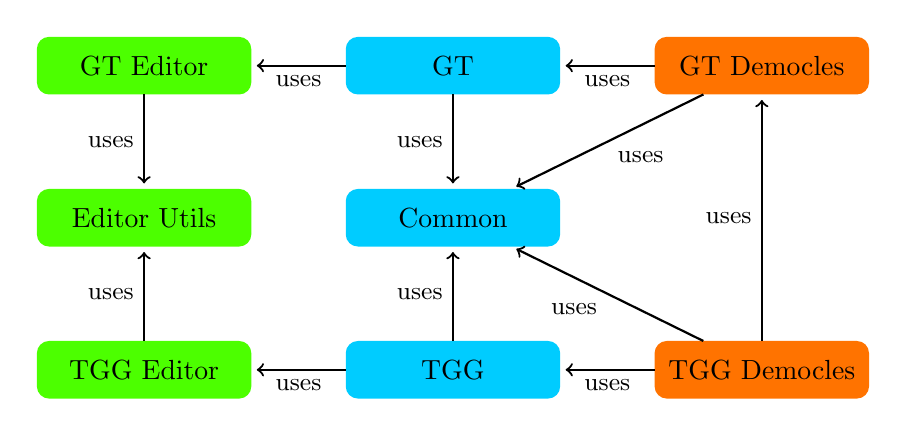
\begin{tikzpicture} [
		auto,
		node/.style = {
			rectangle,
			rounded corners,
			thick,
			text width = 7em,
			text centered,
			minimum height = 2em,
		},
		line/.style = {
			draw,
			thick,
			->,
			shorten >=2pt,
		},
		line-caption/.style = {
			font = \small,
		},
		ibex-ui/.style = {
			draw = green!60!lime,
			fill = green!60!lime,
		},
		ibex/.style = {
			draw = blue!20!cyan,
			fill = blue!20!cyan,
		},
		ibex-democles/.style = {
			draw = red!10!orange,
			fill = red!10!orange
		}
	]

	\matrix[
		column sep = 12mm,
		row sep = 12mm
	] {
		\node[node, ibex-ui] (uiGT) {
			GT Editor
		};
		& \node[node, ibex](GT) {
			GT
		};
		& \node[node, ibex-democles](democlesGT) {
			GT Democles
		};
		\\
		\node[node, ibex-ui] (uiCommon) {
			Editor Utils
		};
		& \node[node, ibex](common) {
			Common
		};
		\\
		\node[node, ibex-ui] (uiTGG) {
			TGG Editor
		};
		& \node[node, ibex](TGG) {
			TGG
		};
		& \node[node, ibex-democles](democlesTGG) {
			TGG Democles
		};
		\\
	};

	\begin{scope} [
		every path/.style = line,
		every node/.style = line-caption
		]
		\path (uiGT) -- node[left] {uses} (uiCommon);
		\path (uiTGG) -- node[left] {uses} (uiCommon);

		\path (GT) -- node {uses} (uiGT);
		\path (TGG) -- node {uses} (uiTGG);

		\path (GT) -- node[left] {uses} (common);
		\path (TGG) -- node[left] {uses} (common);

		\path (democlesGT) -- node {uses} (GT);
		\path (democlesGT) -- node {uses} (common);
		\path (democlesTGG) -- node {uses} (common);
		\path (democlesTGG) -- node {uses} (TGG);
		\path (democlesTGG) -- node {uses} (democlesGT);
	\end{scope}
\end{tikzpicture}
